\documentclass[tikz,border=2pt]{standalone}
\usepackage{pgfplots}
\pgfplotsset{compat=newest}
\begin{document}


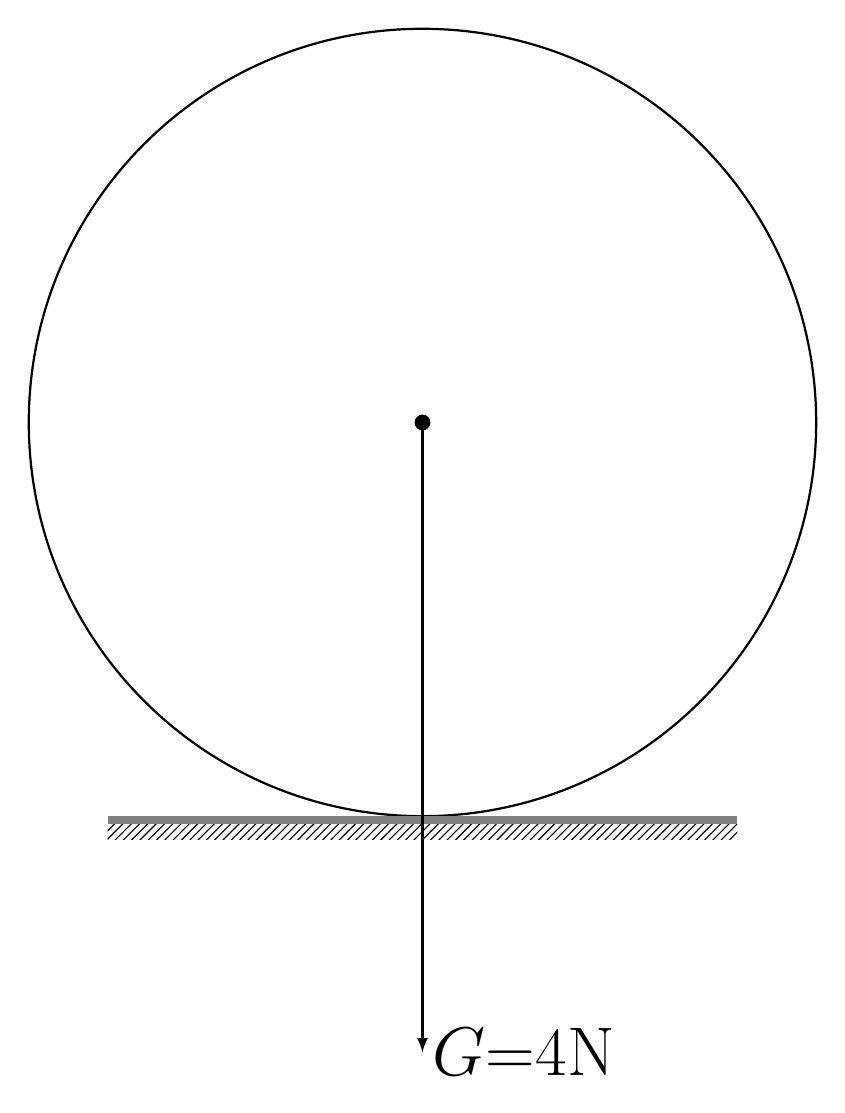
\begin{tikzpicture}[thick]
\newcommand{\ground}[2][]{
\begin{scope}[#1]
\usetikzlibrary{patterns,calc}
\def\groundlen{#2}
\fill[pattern = north east lines] (-#2,0) rectangle (#2,0.2);
\fill[color=black!50] (-#2,0.2) rectangle (#2,0.3);
\end{scope}}
\fill (0,0) circle (0.1);
\draw (0,0) circle (5);

\ground[yshift=-5.3cm]{4cm}

\draw[-latex] (0,0) -- (0,-8) node[right] {\Huge $G$=4N};

\end{tikzpicture}

\end{document}